\input{../header}
\usepackage{pgfplots}
\rhead{Your name: \rule{8cm}{0.15mm}}

\everymath{\displaystyle}
\begin{document}
%


%\onehalfspacing
\allowdisplaybreaks
%##################################################################
\section{Chapter 3 checkpoint!}

Chapter 3 scorecard:
\begin{center}
    \begin{tabular}{|m{3.75cm}|*{4}{m{2.5cm}|}} \hline
        Learning target: & 
        Why derivatives? &
        3.1 &
        3.3 &
        3.6 \\\hline
        Your confidence level before starting (0-5): & &&&\\\hline
        Your confidence level after the quiz (0-5):  & &&&\\\hline
        The mark you earned on this attempt: 
        & Success! \newline Try again!
        & Success! \newline Try again!
        & Success! \newline Try again!
        & Success! \newline Try again!\\\hline

    \end{tabular}
\end{center}

Before anything else, please do the following:
\begin{itemize}
    \item Rank your confidence.
    \item Separate the pages and make sure your name is on each one.
\end{itemize}

Then do the quiz! Some reminders:
\begin{itemize}
    \item Open notes, closed computer.
    \item If you need more room to write, use the back of the same learning target page, or ask me for some scratch paper.
    \item Read the questions carefully and make sure you're answering each part.
    \item Use good grammar for derivative problems.
    \item Show all your work and explain all your thinking!
\end{itemize}
 

Have fun and do your best! I believe in u $\heartsuit$


%%%%%%%%%%%%%%%%%%%%%%%%%%%%%%%%%%%%%%%%%%%%%%%%%%%%%%%%%
\pagebreak
%%%%%%%%%%%%%%%%%%%%%%%%%%%%%%%%%%%%%%%%%%%%%%%%%%%%%%%%%

\section{Applied optimization recipe}

\begin{enumerate}[leftmargin=15pt]
    \item Draw (at least) three pictures.
    \item Decide what quantities are variables and constants. 
    \begin{itemize}
        \item In your pictures, label variables with letters and constants with numbers.
    \end{itemize}
    \item Write down a \textit{constraint equation}. (What keeps you from using whatever numbers you want?)
    \item Write down an \textit{objective function}. (What do you want to be the biggest / smallest possible?)
    \begin{itemize}
        \item Must be a function of one variable only; use your constraint equation to remove extras.
        \item Creativity! Geometry! Trigonometry! Other math you remember!
    \end{itemize}
    \item Figure out any \textit{endpoints}. (Can your one variable be any number you want?)
    \item Do the \textit{finding extrema recipe}:
    \begin{enumerate}
        \item Find all the critical \textit{numbers} of the objective function.
        \item Find all the critical \textit{values} of the objective function.
        \item Find all the endpoint values of the objective function.
        \item Decide who is the smallest and the largest.
    \end{enumerate}

\end{enumerate}

\hrulefill

\section{Related rates recipe}

\begin{enumerate}[leftmargin=15pt]
    \item Draw (at least) three pictures.
    \item Determine what quantities are variables and constants.
    \begin{itemize}
        \item In your pictures, label variables with letters and constants with numbers.
    \end{itemize}
    \item Write down what you know and what you want to know.
    \begin{itemize}
        \item Use good derivative grammar, \(\dfrac{d\square}{dt}\), to label any rates.
        \item Make a note of what things are \textit{always} true and what things are only true \textit{at an instant}.
    \end{itemize}
    \item Write down an equation relating the variables.
    \begin{itemize}
        \item Creativity! Geometry! Trigonometry! Other math you remember!
    \end{itemize}
    \item Find the derivative, \textit{\textbf{with respect to time!!}}, of both sides.
    \item Substitute in the values you know; solve for the rate you want.

\end{enumerate}

%%%%%%%%%%%%%%%%%%%%%%%%%%%%%%%%%%%%%%%%%%%%%%%%%%%
\pagebreak
%%%%%%%%%%%%%%%%%%%%%%%%%%%%%%%%%%%%%%%%%%%%%%%%%%%

\section{Derivatives in related rates vs. applied optimization}

\begin{enumerate}[leftmargin=15pt]
    \item Why are derivatives useful for \textbf{both} related rates problems and applied optimization problems?
    \vfill
    \item What are the most important \textbf{differences} between how derivatives are used in related rates problems vs. applied optimization problems?
    \vfill
\end{enumerate}

%%%%%%%%%%%%%%%%%%%%%%%%%%%%%%%%%%%%%%%%%%%%%%%%%%%
\pagebreak
%%%%%%%%%%%%%%%%%%%%%%%%%%%%%%%%%%%%%%%%%%%%%%%%%%%

\section{Learning target 3.3, version 1}

Write a short but complete answer to each of these questions. Three words is probably incomplete; five sentences is probably too long.
\begin{enumerate}[leftmargin=15pt]
    \item What is a critical number, how do you find them, and why is that how you find them?
    \vfill
    \item What's the difference between a critical \textit{number}, a critical \textit{value}, and a critical \textit{point}?
    \vfill
    \item What's a \textit{sign chart}, and how do you use one to decide what kind of critical point you have?
    \vfill
    \item What's the difference between \textit{relative} or \textit{local} extrema and \textit{absolute} or \textit{global} extrema?
    \vfill
    \item If you have a continuous function on a particular domain, where might its absolute extrema be?
    \vfill
\end{enumerate}

%%%%%%%%%%%%%%%%%%%%%%%%%%%%%%%%%%%%%%%%%%%%%%%%%%%
\pagebreak
%%%%%%%%%%%%%%%%%%%%%%%%%%%%%%%%%%%%%%%%%%%%%%%%%%%

\section{Learning target ??, version 1} % 3.1

Suppose an oil spill in the ocean formed a circle and was growing at a rate of \(53\) feet\(^2/\)minute. When the oil spill reaches a radius of \(35\) feet, how fast is the radius of the oil spill growing? 

\vspace{1em}

Circle what kind of problem this is: \qquad Related rates \qquad Applied optimization

\vspace{1em}

Make sure to do all six steps of the appropriate recipe.

%%%%%%%%%%%%%%%%%%%%%%%%%%%%%%%%%%%%%%%%%%%%%%%%%%%%%%%%%
\pagebreak
%%%%%%%%%%%%%%%%%%%%%%%%%%%%%%%%%%%%%%%%%%%%%%%%%%%%%%%%%
(This side is intentionally blank in case you need more room.)
%%%%%%%%%%%%%%%%%%%%%%%%%%%%%%%%%%%%%%%%%%%%%%%%%%%%%%%%%
\pagebreak
%%%%%%%%%%%%%%%%%%%%%%%%%%%%%%%%%%%%%%%%%%%%%%%%%%%%%%%%%

\section{Learning target ??, version 1} %3.6

You are a dinosaur rancher, and you need to build pens for your three dinosaurs. You decide to build an electric fence around a rectangular region with total area of 30 square kilometers, and then separate this region into three equal-size rectangular pens (10 km$^2$ each) with two more strips of electric fence. What's the minimum length of electric fencing you need to do this? 

\vspace{1em}

Circle what kind of problem this is: \qquad Related rates \qquad Applied optimization

\vspace{1em}

Make sure to do all six steps of the appropriate recipe. Here is one of your three pictures.
\[
	\begin{tabular}{|l|c|c|}
		\hline
 		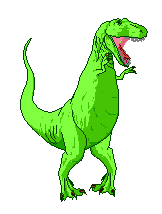
\includegraphics[width=1in]{../images/t-rex.png} & 
 		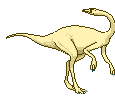
\includegraphics[width=1in]{../images/dromiceiomimus.png} &
 		
\includegraphics[width=1in]{../images/utahraptor.png} \\
		\hline
		% I need a padding row
		\multicolumn{1}{l}{} & \multicolumn{1}{l}{} & \multicolumn{1}{l}{} 
	\end{tabular}
\]
\vfill

%%%%%%%%%%%%%%%%%%%%%%%%%%%%%%%%%%%%%%%%%%%%%%%%%%%%%%%%%
\pagebreak
%%%%%%%%%%%%%%%%%%%%%%%%%%%%%%%%%%%%%%%%%%%%%%%%%%%%%%%%%
(This side is intentionally blank in case you need more room.)


\iffalse

The minimum length of fence is $\underbrace{\qquad\qquad}_{\text{number}}$ $\underbrace{\quad}_{\text{units}}$, 

and the dimensions of the dinosaur pen that make this work are 
$\underbrace{\qquad\qquad}_{\text{number}}\, 
\underbrace{\quad}_{\text{units}}
\times 
\underbrace{\qquad\qquad}_{\text{number}}\,
\underbrace{\quad}_{\text{units}}$.


\section{Learning target AD8, version 1}

A tiger is on the opposite side of a river from a cantaloupe that it wishes to ambush and devour: 

\begin{center}
    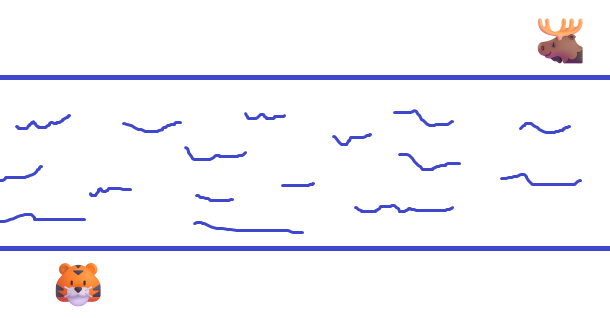
\includegraphics[width=0.8\textwidth]{../images/river-tiger-cantaloupe.png}    
\end{center}

The river is 25 feet wide, and the cantaloupe is 120 feet downstream of the tiger. To get to the cantaloupe, the tiger will have to swim diagonally across the river, then get out and run down the bank.
\fi




\end{document}